% Autor: Alex Oster, Jonathan Sigrist
% Datum: 2018-01
% basiert auf der Vorlage für Versuchsprotokolle von Simon May

\documentclass[
	a4paper,                % Papierformat (DIN A4)
	titlepage=firstiscover, % Separate Titelseite
	captions=tableheading,  % \caption bei Tabellen immer als Überschrift setzen
	toc=bibliography,       % Literaturverzeichnis im Inhaltsverzeichnis aufführen
	toc=listof,             % Abbildungsverzeichnis etc. im Inhaltsverzeichnis aufführen
	oneside,                % Einseitig
	%twoside,               % Zweiseitig
	%twocolumn,             % Zweispaltig
	automark,               % Abschnittstitel automatisch in Kopfzeile einfügen
	12pt,                   % Schriftgröße (beliebige Größen mit „fontsize=Xpt“)
	english, ngerman,       % Sprache für z.B. Babel; ausgewählt: ngerman (letztgenannt)
	%draft=true             % Entwurf-Modus; markiert zu lange und zu kurze Zeilen
]{scrartcl}

% Autor: Simon May
% Datum: 2017-10-04

% --- Pakete einbinden
% --- Pakete erweitern LaTeX um zusätzliche Funktionen.
%     Dies ist ein Satz nützlicher Pakete.

% Silbentrennung etc.; Sprache wird durch Option bei \documentclass festgelegt
\usepackage{babel}
\usepackage{iftex}
\ifLuaTeX
	% Schriftart (Latin Modern)
	\usepackage{fontspec}
	\fontspec{Latin Modern Roman}
\else
	% Verwendung der Zeichentabelle T1 (für Sonderzeichen etc.)
	\usepackage[T1]{fontenc}
	% Legt die Eingabe-Zeichenkodierung fest, z.B. UTF-8
	\usepackage[utf8]{inputenc}
	% Schriftart (Latin Modern)
	\usepackage{lmodern}
	% Zusätzliche Sonderzeichen
	\usepackage{textcomp}
\fi

% Nutzen von +, -, *, / in \setlength u.ä. (z.B. \setlength{\a + 3cm})
\usepackage{calc}
% Wird benötigt, um \ifthenelse zu benutzen
\usepackage{xifthen}
% Optionen für eigene definierte Befehle
\usepackage{xparse}

% Verbessertes Aussehen des Schriftbilds durch kleine Anpassungen
\usepackage{microtype}
% Automatische Formatierung von Daten
\usepackage[useregional]{datetime2}
% Wird für Kopf- und Fußzeile benötigt
\usepackage{scrlayer-scrpage}
% Einfaches Wechseln zwischen unterschiedlichen Zeilenabständen
\usepackage{setspace}
% Optionen für Listen (enumerate, itemize, …)
\usepackage{enumitem}
% Automatische Anführungszeichen
\usepackage{csquotes}
% Zusätzliche Optionen für Tabellen (tabular)
\usepackage{array}

% Mathepaket (intlimits: Grenzen über/unter Integralzeichen)
\usepackage[intlimits]{amsmath}
% Mathe-Symbole, \mathbb etc.
\usepackage{amssymb}
% Weitere Mathebefehle
\usepackage{mathtools}
% „Schöne“ Brüche im Fließtext
\usepackage{xfrac}
% Ermöglicht die Nutzung von \SI{Zahl}{Einheit} u.a.
\usepackage{siunitx}
% Definition von Unicode-Symbolen; Nach [utf8]inputenc laden!
\usepackage{newunicodechar}
% Unicode-Formeln mit pdfLaTeX
% Autor: Simon May
% Datum: 2015-03-04

% Diese Datei ermöglicht es, Mathe-Symbole (z.B. \gamma) direkt als
% Sonderzeichen (d.h. γ) einzugeben

% silence unterdrückt Warnungen; vor hyperref laden
\usepackage{silence}
\WarningFilter[pdflatex-unicode-math]{newunicodechar}{Redefining Unicode character}
\ActivateWarningFilters[pdflatex-unicode-math]

\newunicodechar{†}{\dag}
\newunicodechar{‡}{\ddag}
\newunicodechar{…}{\ldots}
\newunicodechar{⋯}{\cdots}
\newunicodechar{⋮}{\vdots}
\newunicodechar{⋱}{\ddots}
\newunicodechar{⋰}{\iddots}
\newunicodechar{α}{\alpha}
\newunicodechar{β}{\beta}
\newunicodechar{γ}{\gamma}
\newunicodechar{δ}{\delta}
\newunicodechar{ε}{\varepsilon}
\newunicodechar{ϵ}{\epsilon}
\newunicodechar{ζ}{\zeta}
\newunicodechar{η}{\eta}
\newunicodechar{θ}{\theta}
\newunicodechar{ϑ}{\vartheta}
\newunicodechar{ι}{\iota}
\newunicodechar{κ}{\kappa}
\newunicodechar{ϰ}{\varkappa}
\newunicodechar{λ}{\lambda}
\newunicodechar{μ}{\mu}
\newunicodechar{ν}{\nu}
\newunicodechar{ξ}{\xi}
\newunicodechar{ο}{o}
\newunicodechar{π}{\pi}
\newunicodechar{ρ}{\rho}
\newunicodechar{ϱ}{\varrho}
\newunicodechar{σ}{\sigma}
\newunicodechar{τ}{\tau}
\newunicodechar{υ}{\upsilon}
\newunicodechar{φ}{\varphi}
\newunicodechar{ϕ}{\phi}
\newunicodechar{χ}{\chi}
\newunicodechar{ψ}{\psi}
\newunicodechar{ω}{\omega}
\newunicodechar{Α}{\mathrm{A}}
\newunicodechar{Β}{\mathrm{B}}
\newunicodechar{Γ}{\Gamma}
\newunicodechar{Δ}{\Delta}
\newunicodechar{Ε}{\mathrm{E}}
\newunicodechar{Ζ}{\mathrm{Z}}
\newunicodechar{Η}{\mathrm{H}}
\newunicodechar{Θ}{\Theta}
\newunicodechar{Ι}{\mathrm{I}}
\newunicodechar{Κ}{\mathrm{K}}
\newunicodechar{Λ}{\Lambda}
\newunicodechar{Μ}{\mathrm{M}}
\newunicodechar{Ν}{\mathrm{N}}
\newunicodechar{Ξ}{\Xi}
\newunicodechar{Ο}{\mathrm{O}}
\newunicodechar{Π}{\Pi}
\newunicodechar{Ρ}{\mathrm{P}}
\newunicodechar{Σ}{\Sigma}
\newunicodechar{Τ}{\mathrm{T}}
\newunicodechar{Υ}{\Upsilon}
\newunicodechar{Φ}{\Phi}
\newunicodechar{Χ}{\Chi}
\newunicodechar{Ψ}{\Psi}
\newunicodechar{Ω}{\Omega}
\newunicodechar{∑}{\sum}
\newunicodechar{∫}{\int}
\newunicodechar{∬}{\iint}
\newunicodechar{∭}{\iiint}
\newunicodechar{⨌}{\iiiint}
\newunicodechar{∮}{\oint}
\newunicodechar{∯}{\oiint}
\newunicodechar{∰}{\oiiint}
\newunicodechar{∇}{\nabla}
\newunicodechar{∂}{\partial}
\newunicodechar{√}{\sqrt}
\newunicodechar{∈}{\in}
\newunicodechar{∋}{\ni}
\newunicodechar{∉}{\notin}
\newunicodechar{∀}{\forall}
\newunicodechar{∃}{\exists}
\newunicodechar{∄}{\nexists}
\newunicodechar{∴}{\therefore}
\newunicodechar{∵}{\because}
\newunicodechar{〈}{\langle}
\newunicodechar{〉}{\rangle}
\newunicodechar{⌊}{\lfloor}
\newunicodechar{⌋}{\rfloor}
\newunicodechar{⌈}{\lceil}
\newunicodechar{⌉}{\rceil}
\newunicodechar{∼}{\sim}
\newunicodechar{∝}{\propto}
\newunicodechar{∞}{\infty}
\newunicodechar{ℵ}{\aleph}
\newunicodechar{ℏ}{\hbar}
\newunicodechar{℘}{\wp}
\newunicodechar{ℓ}{\ell}
\newunicodechar{∅}{\emptyset}
\newunicodechar{×}{\times}
\newunicodechar{⋅}{\cdot}
\newunicodechar{÷}{\div}
\newunicodechar{⋆}{\star}
\newunicodechar{∘}{\circ}
\newunicodechar{⋄}{\diamond}
\newunicodechar{⊕}{\oplus}
\newunicodechar{⊖}{\ominus}
\newunicodechar{⊗}{\otimes}
\newunicodechar{⊘}{\oslash}
\newunicodechar{⊙}{\odot}
\newunicodechar{±}{\pm}
\newunicodechar{∓}{\mp}
\newunicodechar{≈}{\approx}
\newunicodechar{≡}{\equiv}
\newunicodechar{≠}{\ne}
\newunicodechar{≥}{\ge}
\newunicodechar{≤}{\le}
\newunicodechar{≫}{\gg}
\newunicodechar{≪}{\ll}
\newunicodechar{⊂}{\subset}
\newunicodechar{⊃}{\supset}
\newunicodechar{⊆}{\subseteq}
\newunicodechar{⊇}{\supseteq}
\newunicodechar{⊈}{\nsubseteq}
\newunicodechar{⊉}{\nsupseteq}
\newunicodechar{≔}{\coloneqq}
\newunicodechar{≕}{\eqqcolon}
\newunicodechar{¬}{\neg}
\newunicodechar{∨}{\vee}
\newunicodechar{∧}{\wedge}
\newunicodechar{∪}{\cup}
\newunicodechar{∩}{\cap}
\newunicodechar{⋁}{\bigvee}
\newunicodechar{⋀}{\bigwedge}
\newunicodechar{⋃}{\bigcup}
\newunicodechar{⋂}{\bigcap}
\newunicodechar{⟂}{\perp}
\newunicodechar{∥}{\parallel}
\newunicodechar{∦}{\nparallel}
\newunicodechar{𝚤}{\imath}
\newunicodechar{𝚥}{\jmath}
\newunicodechar{⇔}{\Leftrightarrow}
\newunicodechar{⇕}{\Updownarrow}
\newunicodechar{⇐}{\Leftarrow}
\newunicodechar{⇒}{\Rightarrow}
\newunicodechar{⇑}{\Uparrow}
\newunicodechar{⇓}{\Downarrow}
\newunicodechar{↔}{\leftrightarrow}
\newunicodechar{↕}{\updownarrow}
\newunicodechar{←}{\leftarrow}
\newunicodechar{→}{\rightarrow}
\newunicodechar{↑}{\uparrow}
\newunicodechar{↓}{\downarrow}
\newunicodechar{⟷}{\longleftrightarrow}
\newunicodechar{⟵}{\longleftarrow}
\newunicodechar{⟶}{\longrightarrow}
\newunicodechar{⇇}{\leftleftarrows}
\newunicodechar{⇉}{\rightrightarrows}
\newunicodechar{⇈}{\upuparrows}
\newunicodechar{⇊}{\downdownarrows}
\newunicodechar{⟺}{\Longleftrightarrow}
\newunicodechar{⟸}{\Longleftarrow}
\newunicodechar{⟹}{\Longrightarrow}
\newunicodechar{↦}{\mapsto}
\newunicodechar{↤}{\mapsfrom}
\newunicodechar{⟼}{\longmapsto}
\newunicodechar{⟻}{\longmapsfrom}
\newunicodechar{⟾}{\Longmapsto}
\newunicodechar{⟽}{\Longmapsfrom}
\newunicodechar{↗}{\nearrow}
\newunicodechar{↖}{\nwarrow}
\newunicodechar{↘}{\searrow}
\newunicodechar{↙}{\swarrow}
\newunicodechar{↩}{\hookleftarrow}
\newunicodechar{↪}{\hookrightarrow}
\newunicodechar{↶}{\curvearrowleft}
\newunicodechar{↷}{\curvearrowright}
\newunicodechar{↺}{\circlearrowleft}
\newunicodechar{↻}{\circlearrowright}
\newunicodechar{↫}{\looparrowleft}
\newunicodechar{↬}{\looparrowright}
\newunicodechar{⇋}{\leftrightharpoons}
\newunicodechar{⇌}{\rightleftharpoons}
\newunicodechar{↼}{\leftharpoonup}
\newunicodechar{↽}{\leftharpoondown}
\newunicodechar{⇀}{\rightharpoonup}
\newunicodechar{⇁}{\rightharpoondown}
\newunicodechar{↿}{\upharpoonleft}
\newunicodechar{↾}{\upharpoonright}
\newunicodechar{⇃}{\downharpoonleft}
\newunicodechar{⇂}{\downharpoonright}
\newunicodechar{𝔸}{\mathbb{A}}
\newunicodechar{𝔹}{\mathbb{B}}
\newunicodechar{ℂ}{\mathbb{C}}
\newunicodechar{𝔻}{\mathbb{D}}
\newunicodechar{𝔼}{\mathbb{E}}
\newunicodechar{𝔽}{\mathbb{F}}
\newunicodechar{𝔾}{\mathbb{G}}
\newunicodechar{ℍ}{\mathbb{H}}
\newunicodechar{𝕀}{\mathbb{I}}
\newunicodechar{𝕁}{\mathbb{J}}
\newunicodechar{𝕂}{\mathbb{K}}
\newunicodechar{𝕃}{\mathbb{L}}
\newunicodechar{𝕄}{\mathbb{M}}
\newunicodechar{ℕ}{\mathbb{N}}
\newunicodechar{𝕆}{\mathbb{O}}
\newunicodechar{ℙ}{\mathbb{P}}
\newunicodechar{ℚ}{\mathbb{Q}}
\newunicodechar{ℝ}{\mathbb{R}}
\newunicodechar{𝕊}{\mathbb{S}}
\newunicodechar{𝕋}{\mathbb{T}}
\newunicodechar{𝕌}{\mathbb{U}}
\newunicodechar{𝕍}{\mathbb{V}}
\newunicodechar{𝕎}{\mathbb{W}}
\newunicodechar{𝕏}{\mathbb{X}}
\newunicodechar{𝕐}{\mathbb{Y}}
\newunicodechar{ℤ}{\mathbb{Z}}
\newunicodechar{𝒜}{\mathcal{A}}
\newunicodechar{ℬ}{\mathcal{B}}
\newunicodechar{𝒞}{\mathcal{C}}
\newunicodechar{𝒟}{\mathcal{D}}
\newunicodechar{ℰ}{\mathcal{E}}
\newunicodechar{ℱ}{\mathcal{F}}
\newunicodechar{𝒢}{\mathcal{G}}
\newunicodechar{ℋ}{\mathcal{H}}
\newunicodechar{ℐ}{\mathcal{I}}
\newunicodechar{𝒥}{\mathcal{J}}
\newunicodechar{𝒦}{\mathcal{K}}
\newunicodechar{ℒ}{\mathcal{L}}
\newunicodechar{ℳ}{\mathcal{M}}
\newunicodechar{𝒩}{\mathcal{N}}
\newunicodechar{𝒪}{\mathcal{O}}
\newunicodechar{𝒫}{\mathcal{P}}
\newunicodechar{𝒬}{\mathcal{Q}}
\newunicodechar{ℛ}{\mathcal{R}}
\newunicodechar{𝒮}{\mathcal{S}}
\newunicodechar{𝒯}{\mathcal{T}}
\newunicodechar{𝒰}{\mathcal{U}}
\newunicodechar{𝒱}{\mathcal{V}}
\newunicodechar{𝒲}{\mathcal{W}}
\newunicodechar{𝒳}{\mathcal{X}}
\newunicodechar{𝒴}{\mathcal{Y}}
\newunicodechar{𝒵}{\mathcal{Z}}
\newunicodechar{𝕬}{\mathfrak{A}}
\newunicodechar{𝕭}{\mathfrak{B}}
\newunicodechar{𝕮}{\mathfrak{C}}
\newunicodechar{𝕯}{\mathfrak{D}}
\newunicodechar{𝕰}{\mathfrak{E}}
\newunicodechar{𝕱}{\mathfrak{F}}
\newunicodechar{𝕲}{\mathfrak{G}}
\newunicodechar{𝕳}{\mathfrak{H}}
\newunicodechar{𝕴}{\mathfrak{I}}
\newunicodechar{𝕵}{\mathfrak{J}}
\newunicodechar{𝕶}{\mathfrak{K}}
\newunicodechar{𝕷}{\mathfrak{L}}
\newunicodechar{𝕸}{\mathfrak{M}}
\newunicodechar{𝕹}{\mathfrak{N}}
\newunicodechar{𝕺}{\mathfrak{O}}
\newunicodechar{𝕻}{\mathfrak{P}}
\newunicodechar{𝕼}{\mathfrak{Q}}
\newunicodechar{𝕽}{\mathfrak{R}}
\newunicodechar{𝕾}{\mathfrak{S}}
\newunicodechar{𝕿}{\mathfrak{T}}
\newunicodechar{𝖀}{\mathfrak{U}}
\newunicodechar{𝖁}{\mathfrak{V}}
\newunicodechar{𝖂}{\mathfrak{W}}
\newunicodechar{𝖃}{\mathfrak{X}}
\newunicodechar{𝖄}{\mathfrak{Y}}
\newunicodechar{𝖅}{\mathfrak{Z}}

\DeactivateWarningFilters[pdflatex-unicode-math]


% Farben
\usepackage{xcolor}
% Einbinden von Grafiken (\includegraphics)
\usepackage{graphicx}
% .tex-Dateien mit \includegraphics einbinden
\usepackage{gincltex}
% Größere Freiheiten bei Dateinamen mit \includegraphics
\usepackage{grffile}
% Abbildungen im Fließtext
\usepackage{wrapfig}
% Zitieren, Bibliographie (Biber als Bibliographie-Programm verwenden!)
\usepackage[style=verbose, backend=biber]{biblatex}
% Abbildungen nebeneinander (subfigure, subtable)
\usepackage{subcaption}

% Verlinkt Textstellen im PDF-Dokument (sollte am Ende geladen werden)
\usepackage[unicode]{hyperref}
% „Schlaue“ Referenzen (nach hyperref laden!)
\usepackage{cleveref}
%PDF einbinden
%\usepackage{pdfpages}
%Graphiken zeichnen
%\usepackage{tikz}
%\usetikzlibrary{angles,quotes,babel,3d}
% --- Einstellungen
% -- LaTeX/KOMA
% 1,5-facher Zeilenabstand
\onehalfspacing
\recalctypearea
% Schrift bei Bildunterschriften ändern
\addtokomafont{caption}{\small}
\addtokomafont{captionlabel}{\bfseries}
% Nummerierung der Formeln entsprechend des Abschnitts (z.B. 1.1)
\numberwithin{equation}{section}
% „Verwaiste“ Zeilen am Seitenanfang/-Ende stärker vermeiden
\clubpenalty=1000
\widowpenalty=1000
% Auf mehrere Seiten aufgespaltene Fußnoten stärker vermeiden
\interfootnotelinepenalty=3000

% -- csquotes
% Anführungszeichen automatisch umwandeln
\MakeOuterQuote{"}

% -- siunitx
\sisetup{
	locale=DE,
	separate-uncertainty,
	output-product=\cdot,
	quotient-mode=fraction,
	per-mode=fraction,
	fraction-function=\sfrac
}

% -- hyperref
\hypersetup{
	% Links/Verweise mit Kasten der Dicke 0.5pt versehen
	pdfborder={0 0 0.5}
}

% -- cleveref
\crefname{equation}{}{}
\Crefname{equation}{}{}

% -- biblatex (Literaturverzeichnis)
\IfFileExists{res/literatur.bib}{
	\addbibresource{res/literatur.bib}
}{}

\AtEndPreamble{
	% Kopf- und Fußzeile konfigurieren
	\ifthenelse{\boolean{showHeader}}{
		\KOMAoptions{headsepline}
		\recalctypearea
		\automark{section}
		% Innenseite der Kopfzeile
		\ihead{\headmark}
		% Mitte der Kopfzeile
		\chead{}
		% Außenseite der Kopfzeile
		\ohead{\usekomafont{pagehead}\varAutor}
	}{}
	% Innnenseite der Fußzeile
	\ifoot{}
	% Mitte der Fußzeile          
	\cfoot{-~\pagemark~-}
	% Außenseite der Fußzeile
	\ofoot{}

	% Metadaten für die PDF-Datei
	\hypersetup{
		pdftitle={Versuchsprotokoll: \varName},
		pdfauthor={\varAutor},
		pdfsubject={Grundpraktikum},
		pdfkeywords={Physik, Münster, Praktikum, Versuchsprotokoll}
	}
}


% Autor: Simon May
% Datum: 2017-10-05

% Eigene Befehle eignen sich gut, um Abkürzungen für lange Befehle zu erstellen.
% So vermeidet man, dass man immer wieder dasselbe Konstrukt kopieren und
% einfügen muss und, wenn man dann doch etwas ändern will, an zahllosen Stellen
% im Dokument dieselbe Änderung vornehmen muss.
% Die Syntax ist die folgende:
% \newcommand{neuer Befahl}[Anzahl Parameter (optional)]{Inhalt}
% Das folgende Beispiel fügt ein Bild mit bestimmten vorgegebenen Optionen ein:
\newcommand{\centeredImage}[1]{
	\begin{figure}
		\centering
		\includegraphics[width=0.5\textwidth]{#1}
	\end{figure}
}
% #1 ist dabei ein Parameter, den man \centeredImage übergeben muss, also:
% \centeredImage{...}
% Benötigt man keine Parameter, dann lässt man [1] weg. Werden zusätzliche
% Parameter benötigt, dann kann man die Zahl auf maximal 9 erhöhen.

% Ein Befehl, um eine E-Mail-Adresse darzustellen bzw. automatisch zu verlinken
\newcommand{\email}[1]{\href{mailto:#1}{\texttt{#1}}}

% \arsinh etc.
\newcommand*{\arsinh}{\operatorname{arsinh}}
\newcommand*{\arcosh}{\operatorname{arcosh}}
\newcommand*{\artanh}{\operatorname{artanh}}
\newcommand*{\const}{\text{const.}}

% Autor: Simon May
% Datum: 2016-10-13
% Der Befehl \newcommand kann auch benutzt werden, um „Variablen“ zu definieren:

% Nummer laut Praktikumsheft:
\newcommand*{\varNum}{A2}
% Name laut Praktikumsheft:
\newcommand*{\varName}{Franck-Hertz-Versuch}
% Datum der Durchführung (Format: JJJJ-MM-TT):
\newcommand*{\varDatum}{25.04.2018}
% Autoren des Protokolls:
\newcommand*{\varAutor}{Alex Oster, Jonathan Sigrist}
\newcommand*{\varNameA}{Alex Oster}
\newcommand*{\varNameB}{Jonathan Sigrist}
% Nummer der eigenen Gruppe:
\newcommand*{\varGruppe}{Gruppe Mi 11}
% E-Mail-Adressen der Autoren (kommagetrennt ohne Leerzeichen!):
\newcommand{\varEmail}{a\_oste16@uni--muenster.de,j\_sigr01@uni--muenster.de}
\newcommand{\varEmailA}{a\_oste16@uni--muenster.de}
\newcommand{\varEmailB}{j\_sigr01@uni--muenster.de}
%betreuer Name
\newcommand{\varBetreuer}{\normalsize betreut von \\ Marcel Holtmann}
% E-Mail-Adresse anzeigen (true/false):
\newcommand*{\varZeigeEmail}{true}
% Kopfzeile anzeigen (true/false):
\newcommand*{\varZeigeKopfzeile}{true}
% Inhaltsverzeichnis anzeigen (true/false):
\newcommand*{\varZeigeInhaltsverzeichnis}{true}
% Literaturverzeichnis anzeigen (true/false):
\newcommand*{\varZeigeLiteraturverzeichnis}{true}



\newboolean{showEmail}
\setboolean{showEmail}{\varZeigeEmail}
\newboolean{showHeader}
\setboolean{showHeader}{\varZeigeKopfzeile}
\newboolean{showTOC}
\setboolean{showTOC}{\varZeigeInhaltsverzeichnis}
\newboolean{showBibliography}
\setboolean{showBibliography}{\varZeigeLiteraturverzeichnis}

\renewcommand\maketitle{}

\bibliography{res/literatur}	

\begin{document}
	
	% Römische Seitenzahlen für Titelseite/Inhaltsverzeichnis
	\pagenumbering{roman}
	% Zunächst ohne Kopf-/Fußzeile
	\pagestyle{scrplain}
	
	% --- Titelseite einbinden
	%     Falls die Datei „res/titelbild.pdf“ existiert, wird sie auf der Titelseite
	%     eingefügt
	\IfFileExists{tex/04_Titelseite.tex}{
		% Autor: Simon May
% Datum: 2017-10-05

% Befehl, um die E-Mail-Adressen auf der Titelseite darzustellen
\makeatletter
\newcommand*{\protokollemailparse}[1]{%
	\@for\@tempa:=#1\do{%
		\normalsize\email{\@tempa}\\
	}%
}
\makeatother

<<<<<<< HEAD
\begin{titlepage}
	\centering
	{\scshape\LARGE Versuchsbericht zu \par}
	\vspace{1cm}
	{\scshape\huge \varNum {} --\varName\par}
	\vspace{2.5cm}
	{\LARGE \varGruppe\par}
	\vspace{0.5cm}
	{\large Alex Oster (a\_oste16@uni--muenster.de) \par}
	{\large Jonathan Sigrist (j\_sigr01@uni--muenster.de) \par}
	\vfill
	durchgeführt am \varDatum\par
=======
\title{Versuchsprotokoll \varNum}
\subtitle{\varName}
\subject{Experimentelle Übungen~I}
\date{\DTMdate{\varDatum}}
\ifthenelse{\boolean{showEmail}}{%
	\author{\varAutor\\\normalsize\varGruppe\\\protokollemailparse{\varEmail} \varBetreuer}%
}{%
	\author{\varAutor\\\normalsize\varGruppe \\ \varBetreuer}%
}

>>>>>>> 6ccc0c3e1ae16409205b83e2acdd59de8e60f867

	{\large \varBetreuer} 
	\vfill	
	{\large \today\par}
\end{titlepage}


% Falls die Datei „res/titelbild.pdf“ existiert, wird sie hier eingefügt
\IfFileExists{res/titelbild.pdf}{
	\publishers{\vspace{2ex}
\includegraphics[width=0.75\textwidth]{res/titelbild.pdf}}
}{}

\maketitle

	}{}

	
	% --- Inhaltsverzeichnis einbinden
	\ifthenelse{\boolean{showTOC}}{
		\tableofcontents
		\clearpage
	}{}
	
	% Zurücksetzen der Seitenzahlen auf arabische Ziffern
	\pagenumbering{arabic}
	% Ab hier mit Kopf- und Fußzeile
	\pagestyle{scrheadings}
	
	\newpage
	
	% --- Den Inhalt der Arbeit einbinden
	% --- Kurzfassung des gesammten Berichts (abstract)
	
\section{Kurzfassung}

Dieser Bericht beschäftigt sich mit der Untersuchung von Widerständen und Leistungsabgabe von Verbrauchern. 
Dazu werden zwei Teilversuche betrachtet. In beiden werden die Sachverhalte, die die Theorie liefert bestätigt.

Der Erste beschäftigt sich mit der Untersuchung der Innenwiderstände und der Leistungsabgabe von Akkumulatorzellen.
Zur Betrachtung dieser wird ein einfacher Schaltkreis mit diesen und einem äußeren Widerstand herangezogen.
Durch Messung der anliegenden Spannung in Abhängigkeit des angelegten Widerstandes und der Theorie werden dann die Zusammenhänge aus gemessener und ermittelter Leerlaufspannung gebildet, der Innenwiderstand und die Leistungsabgabe bestimmt.
Das Ziel des Versuches ist die Übereinstimmung der gemessenen Werte mit den ermittelten. 
Dies wird bestätigt, da die gemessene Leerlaufspannung von z.B. \SI{1,2+-0,2}{V} für eine einzelne Akkumulatorzelle mit dem ermittelten Wert von \SI{1,260+-0,194}{V} übereinstimmt. Auch die Werte für drei in Reihe bzw. parallel geschaltete Akkumulatorzellen und für die maximale Leistung stimmen mit den Erwartungen überein.

Der zweite Teilversuch beschäftigt sich mit der Untersuchung des Verhaltens von verschiedenen Verbrauchern bei Gleich- und Wechselstrom.
Dazu werden verschiedene Verbraucher an einen Schaltkreis geschlossen.
Es werden die bei den verschieden Strömen erhaltenen Spannungen, Stromstärken und Leistungen verglichen und Beziehungen mit der Theorie, insbesondere der Impedanzen für die Spule und den Kondensator, sowie dessen Kapazität behandelt. 
Die Theorie zu bestätigen ist das Ziel dieses Versuches.
Dies wird auch anhand der Ergebnisse gezeigt.
Das Verhältnis der Widerstände bei Gleich- und Wechselstrom stimmt mit den Erwartungen überein und die ermittelte Kapazität des Kondensators entspricht bis auf eine kleine Unsicherheit exakt der angegebenen. \SI{0,060+-0,004}{\milli\farad} waren angegeben und \SI{0,060+-0,001}{\milli\farad} wurden ermittelt. 


	\vspace{2cm}

	% --- Einzelne Teilversuche einbinden
	\clearpage
	\section{Untersuchung von Akkumulatorzellen} 

% TODO
% Dies ist ein Teilversuch.
% Der Abschnitt sagt grundsätzliches über den konkreten Versuch aus.
% Es werden relevante physikalische Effekte qualitativ beleuchtet.
% Es wird das Ziel des Versuchs angegeben.

% Die Ergebnisse werden kurz, aber mit konkreten Werten erwähnt.
% Dann werden diese in den Kontext kurz eingebunden.

\subsection{Methoden}

\subsubsection{Aufbau}

Der Aufbau dieses Versuchs beschränkt sich auf einen simplen Schaltkreis, welcher zunächst nur aus einer Akkumulatorzelle und einem regulierbaren Widerstand $R_a$ besteht. 
Zusätzlich dazu ist ein Multimeter an die Akkumulatorzelle geschlossen, sodass die dort anliegende Spannung gemessen werden kann. 
Mit diesem Aufbau wird zuerst die Leerlaufspannung $U_0$ der Akkumulatorzelle und dann der Innenwiderstand $R_i$ dieser bestimmt.
Dazu wird die Klemmspannung $U_{kl}$ gemessen und in Abhängigkeit des elektrischen Stroms $I$ gesetzt, welcher sich durch die Spannung und dem anliegenden Widerstand bestimmen lässt.

Dieser Vorgang wird dann für drei in Reihe- und drei parallel geschaltete Akkumulatorzellen wiederholt. 

\subsubsection{Unsicherheiten}

Bei diesem Versuch treten lediglich die Unsicherheit des Multimeters und des Lastwiderstands $R_a$ auf. 
Da das Multimeter eine analoge Darstellung der Messwerte verwendet und sich je nach verwendeter Größenordnung mit einer Genauigkeit von \SI{1}{V} bzw. \SI{0,1}{V} ablesen ließ, werden die zugehörigen Unsicherheiten über eine Dreiecksverteilung bestimmt.
Für die Unsicherheit des Widerstands wird, da es sich hierbei um einen alten Stöpselwiderstand, eine prozentuale Abweichung des angegebenen Werts von 10\% gewählt.
Im Allgemeinen werden zur Berechnung der kombinierten Unsicherheiten die nach GUM vorgesehenen Formeln verwendet. 
Die Berechnung dieser für diesen Versuch erfolgt im Anhang (\ref*{sec:anhang}).

\subsection{Datenanalyse}

Alle aufgenommenen Werte sind dem Laborbuch zu entnehmen. 
Darüber hinaus sind die Daten in den folgenden Diagrammen graphisch dargestellt.

Zur Bestimmung der Leerlaufspannung wird ein "unendlich" großer Widerstand gewählt, der Stromkreis also nicht geschlossen.
Für diese ergeben sich \SI{1,2+-0,2}{V} für die einzelne Akkumulatorzelle, \SI{3,7+-0,2}{V} drei in Reihe geschaltete Zellen und erneut \SI{1,2+-0,2}{V} drei parallel geschaltete Akkumulatorzellen. 

Da es sich bei der Akkumulatorzelle um keine ideale Spannungsquelle hält, was sich physikalisch auch nicht realisieren lässt, wird sie als Reihenschaltung von idealer Spannungsquelle $U_0$ und Innenwiderstand $R_i$ angenommen. 
Nach dem zweiten Kirchhoff'schen Gesetz folgt mit Belastung eines äußeren Widerstands:
\begin{align}
	U_0 = R_i I + R_a I \\
	\text{und durch umformen nach $R_i$ folgt:} \quad R_i = \frac{U_0}{I}-R_a.
\end{align}
Der elektrische Strom $I$ lässt sich hierbei durch die gemessene Klemmspannung $U_{kl}$ und dem Widerstand $R_a$ ermitteln ($I=\frac{U_{kl}}{R_a}$).
Zu Beachten ist hierbei, dass sich kein Wert für einen Außenwiderstand von \SI{0}{\Omega} ermitteln lässt, da dafür durch null geteilt werden müsste.
In diesem Falle kommt es zum Kurzschluss.
Dabei ist der Strom maximal, aber endlich, kann jedoch zur Rechnung nicht verwendet werden.
Ebenso führt die oben angegebene Formel für einen unendlich großen Außenwiderstand dazu, dass der Innenwiderstand gegen null geht, da sich $U_{kl}$ der Leerlaufspannung $U_0$ annähert und $R_i = R_a - R_a = 0$ übrig bleibt.
Umformen der oberen Gleichung nach der Klemmspannung $U_{kl} = R_a I$ lässt darauf schließen, dass der Innenwiderstand $R_i$ sich auch als Steigung der Gleichung $U_{kl} = -R_i I + U_0$ identifizieren lässt. Dies ist in den Diagrammen \ref{label} bis \ref{label} für die drei Fälle dargestellt\footnote{Die Fits und deren Unsicherheiten wurden von dem Programm SciDavis berechnet, dazu wurden die Unsicherheiten (welche im Anhang zu finden sind) und die Methode der kleinsten Quadrate herangezogen}.
Somit ergibt sich ein Innenwiderstand von \SI{0}{\Omega} für eine einzelne Akkumulatorzelle, \SI{0}{\Omega} für drei in Reihe geschaltet und \SI{0}{\Omega} für drei parallelgeschaltete Zellen. %TODO Messwerte
Daraus folgt, dass sich der Innenwiderstand in einer Größenordnung von \SI{0}{\Omega} befindet. %TODO folgern


% Rechnungsweg zum Ergebnis angeben und begründen, warum z. B. linearer Fit genommen wurde.
% Dazu auf die Theorie oder die Versuchsanleitung Bezug nehmen.
% Vollständige Fehlerberechnung in den Anhang.
% Da grundsätzlich schon vorher erläutert (GUM) reicht hier eine kurze Anmerkung auf die Fehlerrechnung.
% Ergebnis graphisch darstellen und auf passende Darstellungsweise (Unsicherheiten, signifikante Stellen) achten.

% Falls mehrere voneinander unabhängige Lösungen existieren (z. B. bei der geometrischen Bestimmung des Trägheitsmomentes des Kreisels), können diese in Unterkapitel gegliedert werden.

\subsection{Diskussion}

% Die Ergebnisse in den Kontext einbinden.
% Zusammenhänge noch einmal darstellen.
% Jegliche Aussagen durch Ergebnisse oder Vorwissen untermauern.
% Ergebnisse mit Referenzwerten/Literaturwerten vergleichen und auf Unsicherheiten eingehen (Vertrauensgrad).

\subsection{Schlussfolgerung}

% Das Ziel noch einmal erläutern.
% Fazit des Versuchs angeben (untermauert die These; weicht von den Literaturwerten ab; ...).
% Warum folgt aus den Ergebnissen das Fazit.
% Mit ermittelten Daten und Unsicherheiten begründen.
% Auf Unsicherheiten weiter eingehen und Vertrauensgrad bzw. Relevanz der Schlussfolgerung auf die derzeitige Wissenslage angeben (meistens nicht relevant).
% Verbesserungsvorschläge für das nächste Mal und allgemeine Rekapitulierung über das durchgeführte Experiment.
% Warum muss man das Experiment unbedingt noch mal durchführen.

	\IfFileExists{tex/12_Versuch2.tex}{
		\clearpage
		\subsection{Teilversuch 2: $ \lambda  / 2 $-Plättchen}

	\subsubsection*{Methoden}
		
		\begin{figure}[ht]
			\centering
			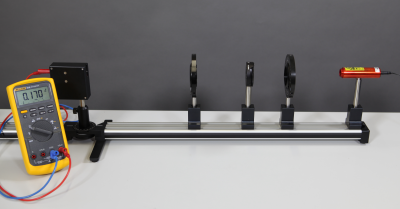
\includegraphics[width=\textwidth]{bilder/LambdaHalbe.png}
			\caption{Aufbau des zweiten Teilversuches.\cite{WWU}}
			\label{fig:LambdaHalbe}	
		\end{figure}
		Der Aufbau des zweiten Teilversuches ist in Abb. \ref{fig:LambdaHalbe} dargestellt.
		Dieser Teilversuch verläuft analog zu dem ersten, nur dass hier zusätzlich das $\lambda/2$-Plättchen zwischen den beiden Polarisatoren platziert wird.
		
		Beim Eintritt in das Plättchen sind der parallele und der orthogonale Teil des E-Feld Vektors in Phase. 
		Nach dem Durchlaufen des doppelbrechenden Plättchens ($n_1 , n_2$) ist aufgrund der unterschiedlichen Laufzeiten der beiden Komponenten eine Phasendifferenz $\Delta\phi$ zwischen ihnen entstanden.
		
		Gilt für die Dicke $d$ des Plättchens $d\cdot(n_2-n_1)=\lambda/2$, so wird $\Delta\phi=\pi$ und der E-Feld Vektor dreht sich um den Winkel $\Delta\alpha = 2\phi$.
		Drehen des $\lambda/2$-Plättchens um einen Winkel $\phi$ führt zu einer Drehung der Polarisationsebene um den doppelten Winkel $2\phi$.
		
		Für diesen Versuch soll das $\lambda/2$-Plättchen gedreht werden und beobachtet werden um welchen Winkel sich das Maximum über Drehung des zweiten Polarisators verschoben hat.
		
	\subsubsection*{Durchführung}
	
		Wie auch bei dem ersten Teilversuch war die gemessene Spannung für die Polarisatoren bei $\phi_{\text{p1}} = \SI{106+-0,4}{\degree}$ maximal.
		Zunächst wurde gesucht, bei welchem Winkel des $\lambda/2$-Plättchens das Maximum bei dem hinteren Polarisator gleich bleibt.
		Dies war bei $\phi_{0,\lambda/2} = \SI{108+-0,8}{\degree}$ der Fall.
		Zur Überprüfung, ob sich der Polarisatorwinkel für das Maximum um das Doppelte des Drehwinkels $\phi_{\lambda/2}$ verschiebt, wurde letzterer auf \SI{152+-0,8}{\degree} gesetzt.
		Daraufhin ließ sich das Maximum an dem zweiten Polarisator bei $\phi_{\text{p2}} = \SI{196+-0,4}{\degree}$ finden.
		Für $\Delta\phi_{\lambda/2} = \SI{44}{\degree}$ ($\approx \SI{45}{\degree}$ in seiner Unsicherheit) findet an dem Polarisator eine Änderung von $\Delta\phi_{\text{p2}} = \SI{90}{\degree}$ statt.
		Ausgehend von dem ursprünglichen Maximum wurden nun für fünf weitere Winkel $\phi_{\lambda/2}$ in \SI{10}{\degree} Schritten die Maximawinkel $\phi_\text{p2}$ aufgezeichnet.
	
	\subsubsection*{Datenanalyse}
		
		\begin{figure}[ht]
			\centering
			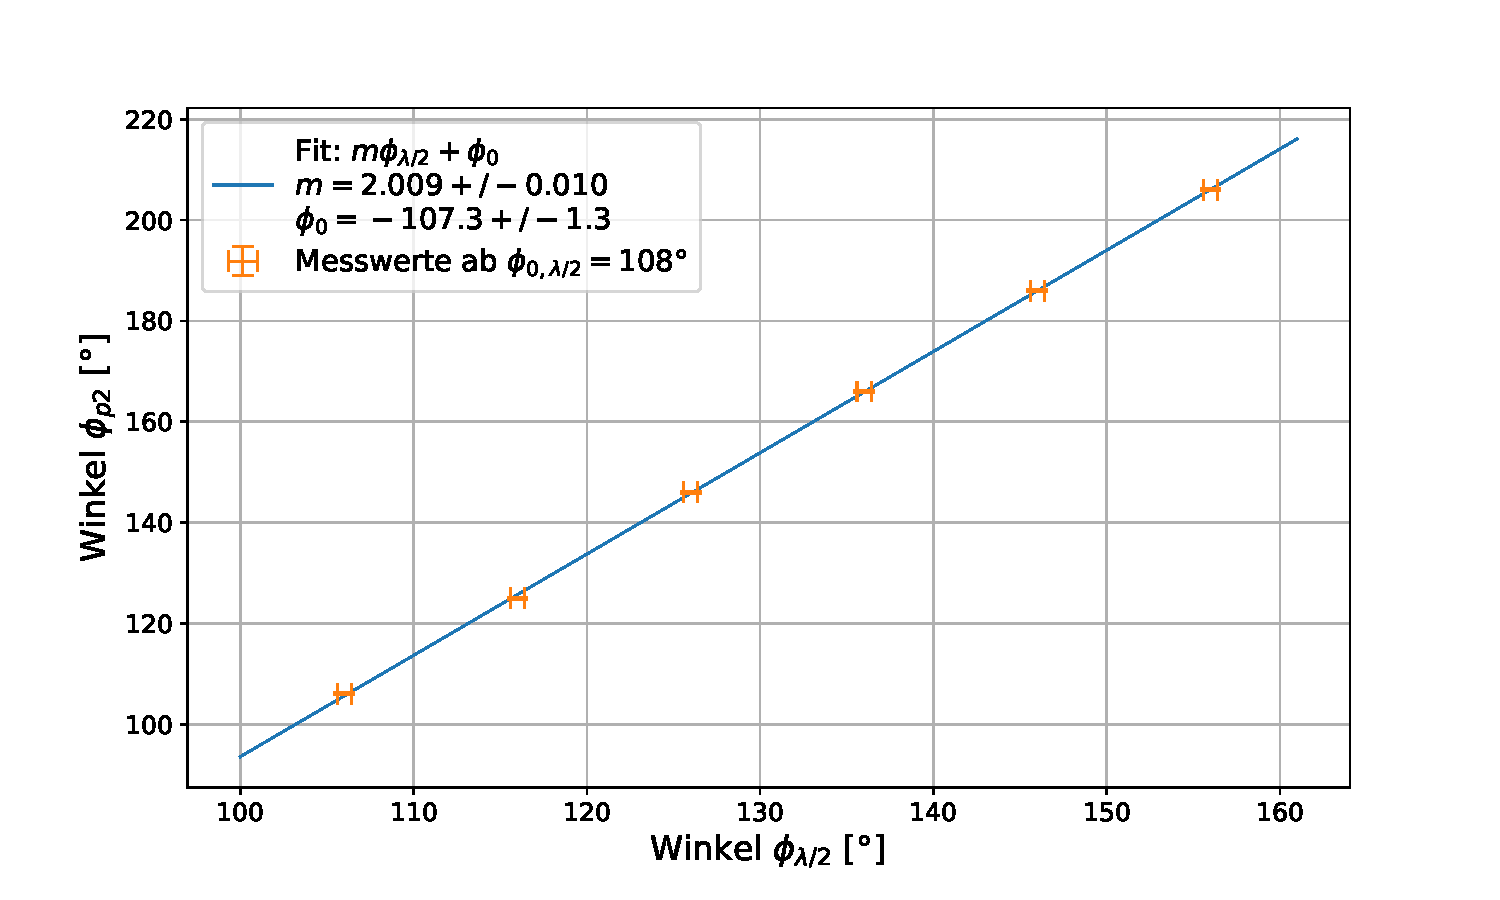
\includegraphics[width=\textwidth]{data/lambdaPolarisation.pdf}
			\caption{Messpunkte und linearer Fit für das Verhältnis $m$ der Winkel $\phi_{\lambda/2}$ und $\phi_{p2}=\phi'$.}
			\label{fig:LambdaHalbeFit}	
		\end{figure}
		Aus den Messpunkten ließ sich das Verhältnis der beiden Winkel $\phi_{\lambda/2}$ und $\phi_{p2}$ genauer bestimmen.
		Da der lineare Faktor zwei zu erwarten war, wurde an dieser Stelle ein linearer Fit verwendet.
		Abb. \ref{fig:LambdaHalbeFit} stellt diesen Verlauf und die Messpunkte dar.
		Die Steigung des Fits beträgt $m = \SI{1,998+-0,006}{}$, 2 liegt somit innerhalb einer Unsicherheit.
	
	\subsubsection*{Diskussion}
	
		Das Ergebnis dieses Teilversuches ist, dass das Verhältnis zwischen den Winkeln $\phi_{\lambda/2}$ und $\phi_{p2}$ gerade \SI{1,998+-0,006}{} entspricht.
		Der Wert ist in Übereinstimmung mit der Hypothese, dass dieses Verhältnis zwei entspricht, da er sich innerhalb der Unsicherheiten des Ergebnisses befindet.
		
	}{}
	\IfFileExists{tex/13_Versuch3.tex}{
		\clearpage
		\subsection{Teilversuch 3: Reflexionsvermögen einer Glasplatte und Brewster Winkel}

	\subsubsection*{Methoden}
		
		\begin{figure}[ht]
			\centering
			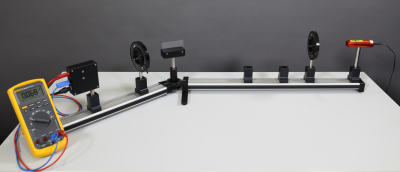
\includegraphics[width=\textwidth]{bilder/Brewster-Winkel.png}
			\caption{Aufbau des dritten Teilversuches\cite{WWU}}
			\label{fig:Glasplatte}	
		\end{figure}
		Der dritte Teilversuch soll wie in Abb. \ref{fig:Glasplatte} dargestellt aufgebaut werden.
		Hier steht statt des $\lambda/2$-Plättchens nun eine Glasplatte in dem Strahlengang.
		Nun soll betrachtet werden wie sich das Reflexionsvermögen der Glasplatte für Einstrahlung von senkrecht bzw. parallel polarisiertem Licht verhält.
		Senkrechtes (s) und paralleles (p) polarisiertes Licht sind die Anteile des polarisierten Lichts, die selbsterklärend senkrecht bzw. parallel zu der Glasplatte eingestrahlt werden.
		Dazu wird die Photodiode an einem Ende und der Laser an dem anderen angebracht, sodass diese an dem beweglichen Gelenk mit der Glasplatte um einen variablen Winkel $\Theta$ versetzt werden können.
		Für die Winkel \SIrange{30}{85}{\degree} soll dafür in \SI{5}{\degree} Schritten die Intensität gemessen werden.
		Besonders ist hierbei der Brewster-Winkel, bei dem der reflektierte und der transmittierte Strahl senkrecht zueinander verlaufen bzw. der E-Feld Vektor ausschließlich senkrecht zu der Einfallsebene schwingt.
		Dadurch spielt in der Messung auch nur der parallele Anteil des Laserlichts eine Rolle.
		Aus dem Snellius'schen Brechungsgesetz folgt für die Brewster-Beziehung dann
		\begin{equation} \label{eq:Brewster}
			\tan{\Theta_\text{B}} = n,
		\end{equation}
		für den Fall dass einer der Brechungsindizes eins entspricht (wie hier bei Luft).
		Die Größe $n$ beschreibt hier dann den Brechungsindex der Glasplatte.

	\subsubsection*{Durchführung}
		
		\begin{figure}[ht]
			\centering
			\includegraphics[width=\textwidth]{data/Spiegel.pdf}
			\caption{Aufgenommene Spannungen in Abhängigkeit des Winkels $\Theta$. Die Spannung ist logarithmisch aufgetragen, um das Minima beim Brewster-Winkel $\Theta_\text{B}$ deutlicher erkennen zu können.}
			\label{fig:GlasplatteWinkel}	
		\end{figure}
		Für die Winkel \SIrange{30+-0,4}{85+-0,4}{\degree} wurden in \SI{5+-0,4}{\degree} die zugehörigen Spannungen an der Photodiode gemessen.
		Diese sind in \ref{fig:GlasplatteWinkel} aufgetragen.
	
	\subsubsection*{Datenanalyse}
		
		Die geringste Spannung unter den Messpunkten ließ sich bei $\Theta = \SI{55+-0,4}{\degree}$ beobachten.
		Damit sollte der Brewster-Winkel für die Glasplatte bei $\Theta_\text{B} =  \SI{55+-0,4}{\degree}$ liegen.
		Einsetzen dieses Winkels in Gl. \ref{eq:Brewster} führt zu dem Brechungsindex $n = \SI{1,5508+-0,0008}{}$ für die Glasplatte.
	
	\subsubsection*{Diskussion}
		
		\begin{figure}[ht]
			\centering
			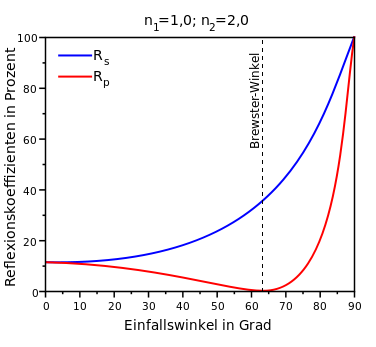
\includegraphics[width=0.6\textwidth]{bilder/wikiBrewster.png}
			\caption{Theoretische Kurve des parallel polarisierten Anteils (rot) bei $n_2 = 2$. \cite{wikiBrewster}}
			\label{fig:wiki_brewster}	
		\end{figure}
		Um zu Überprüfen, ob die gemessenen und ermittelten Werte mit dem bereits bewiesenem Sachverhalt übereinstimmen, dienen die Abb. \ref{fig:wiki_brewster} und Literaturwerte für den Brechungsindex von Glas.
		Vergleicht man zunächst die aufgenommenen Messpunkte aus Abb. \ref{fig:GlasplatteWinkel} mit der theoretischen Kurve aus Abb. \ref{fig:wiki_brewster}, bei der der Brechungsindex $n_2 = n = 2$ ist, so besitzt der Verlauf des gemessenen Anteils eine ähnliche Form wie die der theoretischen (roten) Kurve.
		Da der aus den Messpunkten ermittelte Brechungsindex bei $n = \SI{1,5508+-0,0008}{}$ liegt, ist eine exakte Übereinstimmung mit der Theorie für $n=2$ jedoch auch nicht zu erwarten gewesen.
		Des Weiteren stellt sich die Frage ob der ermittelte Wert für den Brechungsindex der Glasplatte  einen passenden darstellt.
		Für Kronglas dient der Literaturwert\cite{Refrac} von $n = \SI{1.5145}{}$ und für Flintglas $n = \SI{1.6661}{}$.
		Eine genaue Beschreibung, um welches Glas es sich bei der Platte handelte, war nicht gegeben und zu keinem der beiden Literaturwerte liegt eine genaue Übereinstimmung vor.
		Da der $n$ jedoch zwischen beiden liegt, lässt sich zumindest vermuten, dass die Glasplatte tatsächlich aus einem Glas besteht.
		Ein Widerspruch zu den Fresnel'schen Formeln und der Beugungstheorie lässt sich an dieser Stelle nicht finden.
		
		
	}{}
	\IfFileExists{tex/14_Versuch4.tex}{
		\clearpage
		\subsection{Teilversuch 4: Strahlenversatz}

	\subsubsection*{Methoden}
		
		% TODO
		
	\subsubsection*{Durchführung}
	
		% TODO
	
	\subsubsection*{Datenanalyse}
		
		% TODO
	
	\subsubsection*{Diskussion}
	
		% TODO
	}{}
	\IfFileExists{tex/15_Versuch5.tex}{
		\clearpage
		\subsection{Teilversuch 5: Kristallpolarisation}

	\subsubsection*{Methoden}
		
		% TODO
		
	\subsubsection*{Durchführung}
	
		% TODO
	
	\subsubsection*{Datenanalyse}
		
		% TODO
	
	\subsubsection*{Diskussion}
	
		% TODO
	}{}
	%\input{tex/name.tex}
	% --- Fazit des gesammten Versuchs einbinden, falls nötig
	\IfFileExists{tex/19_Fazit.tex}{		
		\section{Schlussfolgerung}
	
	Bis auf die Abweichungen bei Schärfentiefen $S_\text{(sub)}$ bei höheren Blendenzahlen $k$ und dem Lochblenden-Foto ließen sich die restlichen Ziele, zu zeigen dass Blenden einen Einfluss auf das Auflösungsvermögen besitzen, wie auch den Zusammenhang zwischen Blendengröße und Belichtungszeit, erreichen:

	Eine Übereinstimmung zwischen den berechneten Schärfentiefen ließ sich nicht finden.
	Die ersten Werte liegen noch innerhalb einer Unsicherheit voneinander, für größere Blendenzahlen $k$ jedoch wichen die Werte stark voneinander ab.
	Aufgrund der großen Unsicherheiten können diese Abweichungen jedoch nicht als Widerspruch für $Z = D_\text{B}/1500$ gesehen werden.
	
	Des Weiteren ließ sich für das Auflösungsvermögen bestimmen, dass die Blendzahlen $k = 5,6$ und $k = 8$ die kleinsten Halbwertsbreiten und somit die beste Auflösung besitzen; Blenden die Auflösung also verbessern können, indem sie Linsenfehler, welche am Rand auftreten, ausbessern.
	Unter den Blenden war dies insbesondere bei der \SI{3,75}{\milli\meter}-Blende der Fall.
	Neben der MTF-Methode brachte auch die Auswertung über Siemenssterne das gleiche Ergebnis.
	
	Für die zunächst unbestimmte Größe der Lochblende ließ sich durch die Belichtungszeiten eine Approximation auf \SI{0,235+-0,035}{\milli\meter} durchführen. 
	
	Eine Wiederholung des Versuches als Ganzes scheint aufgrund der Ergebnisse nicht sinnvoll, jedoch bietet es sich an aufgrund des Fehlens des Auflösungsvermögens der Lochblende zumindest an dieser Stelle ein neues Foto unter besseren Randbedingungen (Beleuchtung, Schirmabstand etc.) aufzunehmen.
	
	}{}
	
	% --- Anhang einbinden
	\IfFileExists{tex/20_Anhang.tex}{
		\clearpage
		%\appendix
		\section{Anhang}
		\label{sec:anhang}
		\subsection{Unsicherheiten}\label{VGuD}

Jegliche Unsicherheiten werden nach GUM bestimmt und berechnet.
Die Gleichungen dazu finden sich in \ref{fig:GUM_combine} und \ref{fig:GUM_formula}.
Für die Unsicherheitsrechnungen wurde die Python Bibliothek "uncertainties" herangezogen, welche den Richtlinien des GUM folgt.
Alle konkreten Unsicherheitsformeln stehen weiter unten.
Für Unsicherheiten in graphischen Fits wurden die $y$-Unsicherheiten beachtet und die Methode der kleinsten Quadrate angewandt.
Dafür steht in der Bibliothek die Methode "scipy.optimize.curve_fit()" zur Verfügung.


Für digitale Messungen wird eine Unsicherheit von $u(X) = \frac{\Delta X}{2\sqrt{3}}$ angenommen, bei analogen eine von $u(X) = \frac{\Delta X}{2\sqrt{6}}$.

\begin{description}
	\item[Schieblehre] Die Schieblehre hatte eine angegebene analoge Unsicherheit von $\Delta d = \SI{0.05}{\milli\meter}$.
	Mit ihr wurde die Dicke der Separationsscheiben und somit die Spaltdicke sowie der Innendurchmesser des Glasröhrchens gemessen.
		
	\item[Messstab] Hier konnte der Wert mit einer Genauigkeit von $\Delta h = \SI{1}{\milli\meter}$ analog abgelesen werden.
	Die Unsicherheit wurde bei der Höhe des Schlitzes über dem Flaschenrand und bei dem Wasserstand im Manometer verwendet.
	
	\item[Waage] Die Digitalwaage konnte Gewichte auf $\Delta m = \SI{0.1}{\gramm}$ unterscheiden.
	Sie wurde zur Bestimmung des Schwingkörpergewichtes benutzt.
	
	\item[Barometer] Hier ließen sich Werte analog bis auf $\Delta p = \SI{0.1}{\milli\bar}$ ablesen.
	Es wurde bei der Messung des statischen Außendrucks benötigt.
	
	\item[Glasflasche] Das Volumen der Glasflasche war angegeben.
	Dabei wurde eine Unsicherheit von $\Delta V = \SI{10}{\centi\meter\cubed}$ angenommen.
	
	\item[Stopuhr] Die Unsicherheit der Zeitmessung setzt dich aus der analogen Reaktionszeit mit $\Delta t_\text{R} = \SI{0.1}{\second}$ und der digitalen Anzeigegenauigkeit von $\Delta t_\text{Uhr} = \SI{0.01}{\second}$ nach \ref{unc:time} zusammen.
		
\end{description}

\begin{figure}[h]
	\begin{equation*}
		x = \sum_{i=1}^{N} x_i
		;\quad
		u(x) = \sqrt{\sum_{i = 1}^{N} u(x_i)^2}
	\end{equation*}
	\caption{Formel für kombinierte Unsicherheiten des selben Typs nach GUM.}
	\label{fig:GUM_combine}
\end{figure}

\begin{figure}[h]
	\begin{align*}
		f = f(x_1, \dots , x_N)
		;\quad
		u(f) = \sqrt{\sum_{i = 1}^{N}\left(\pdv{f}{x_i} u(x_i)\right) ^2}
	\end{align*}
	\caption{Formel für sich fortpflanzende Unsicherheiten nach GUM.}
	\label{fig:GUM_formula}
\end{figure}

\begin{figure}[h]
	\begin{equation*}
		u(t) = \sqrt{u^2(t_\text{R}) + u^2(t_\text{Uhr})}
	\end{equation*}
	\caption{Formel für Zeitmessungen nach \ref{fig:GUM_combine}.} 
	% sonst: \caption{Formel für Zeitmessungen nach GUM mit Unsicherheiten desselben Typs.}
	\label{unc:time}
\end{figure}

\begin{figure}[h]
	\begin{align*}
		A = \frac{\pi}{4} d^2
		;\quad
		u(A) = \frac{\pi}{2} d u(d)
		}
	\end{align*}
	\caption{Formel für die Fehlerfortpflanzung der Querschnittsfläche des Glasrohrs.}
	\label{unc:querschnitt}
\end{figure}

\begin{figure}[h]
	\begin{align*}
		p_0 = p_{L} + \frac{m g}{A}
		;\quad
		u(p_0) = \sqrt{u^2(p_\text{L}) + \left( \frac{g u(m)}{A}\right)^2 + \left( \frac{m g u(A)}{A^2}\right)^2}
	}
	\end{align*}
	\caption{Fehlerfortpflanzung bei der Dichtekombination..}
	\label{unc:dichte}
\end{figure}

\begin{figure}[h]
	\begin{align*}
		V_0 = V_\text{F} + A \Delta x
		;\quad
		u(V_0) = \sqrt{u^2(V_\text{L}) + u^2(A) (\Delta x)^2 + A^2 u^2(\Delta x)}
	}
	\end{align*}
	\caption{Formel für die Fehlerfortpflanzung des Volumens der Glasflasche. $\Delta x$ ist die Höhe des Schlitzes über dem Flaschenhalz.}
	\label{unc:volumen}
\end{figure}

\begin{figure}[h]
	\begin{align*}
		\kappa = \frac{4 \pi^2 m V}{p_0 A^2 T^2} \\
		u(\kappa) = 4 \pi^2 \sqrt{
			\left( \frac{V}{p_0 A^2 T^2} u(m) \right)^2 + 
			\left( \frac{m}{p_0 A^2 T^2} u(V) \right)^2 + 
			\left( \frac{-m V}{p_0^2 A^2 T^2} u(p_0) \right)^2 + 
			\left( \frac{ -2 m V}{p_0 A^3 T^2} u(A) )^2 + 
			\left( \frac{ -2 m V}{p_0 A^2 T^3} u(T)\right)^2 
		}
	\end{align*}
	\caption{Formel für die Fehlerfortpflanzung bei der Bestimmung von $\kappa$ nach Rückhardt-Flammersfeld.}
	\label{unc:schwingung}
\end{figure}


\begin{figure}[h]
	\begin{align*}
		\kappa = \frac{h_1}{h_1 - h_3} \\
		u(\kappa) = \sqrt{
			\left( -\frac{h_3 u(h_1)}{(h_1 - h_3)^2} \right)^2 + 
			\left( \frac{h_1 u(h_3)}{(h_1 - h_3)^2} \right)^2
		} = \frac{1}{(h_1 - h_3)^2} \sqrt{h_3^2 u^2(h_1) + h_1^2 u^2(h_3)}
	\end{align*}
	\caption{Formel für die Fehlerfortpflanzung bei der Bestimmung von $\kappa$ nach Clément-Desormes.}
	\label{unc:pumpe}
\end{figure}

	}{}
	
	% --- Literaturverzeichnis mit BibLaTeX
	\ifthenelse{\boolean{showBibliography}}{
		\clearpage
		\printbibliography
	}{}
	
\end{document} 
